
\chapter{Preliminary}
In order to understand the topic of variational autoencoders or even autoencoders in general, we need to consider a couple of preliminary ideas. Those ideas consist mainly of neural networks and their optimization - usually being called training. In this chapter, we will tackle the conceptional idea of how to formulate neural networks in a mathematical way and further, we will consider a couple of useful operations that neural networks are capable of doing. Lastly, we will take a look at some strategies of training neural networks.

\section{Neural networks}
Originally, the idea of neural networks originated in analysing mammal's brains. An accumulation of nodes - so called neurons, connected in a very special way that fire an electric impulse to adjacent neurons upon being triggered and transmit information that way. Scientist tried to mimic this natural architecture and replicate the human intelligence artificially. This research has been going for almost 80 years and became immensely popular recently through artificial intelligences like OpenAI's ChatGPT or Google's Bard. But what do these neural networks do? Why are they so popular? What actually is a neural network? All those are very interesting and important questions that we will find answers for.\\
As already mentioned, neural networks consist of single neurons that move around information upon being \glqq triggered\grqq{}. Obviously, triggering an artificial neuron can't happen the same way as neurological neurons are being triggered. Hence, we need to model the triggering of a neuron in some way. The idea is to filter information that does not exceed a certain stimulus threshold. This filter is usually being called activation function. Indeed, there are lots of ways of modelling such activation functions and it primarily depends on the specific use-case what exactly the activation function has to fulfil. Therefore, we define activation functions in the most general way possible.

\begin{definition}
A non-constant function $\f: \R \to \R$ is called an \textbf{activation function} if it is continuous.
\end{definition}

Even though there is a zoo of different activation functions, we want to consider mainly the following ones.

\begin{example}
The following functions are activation functions.
\begin{mydescription}{\widthof{\textbf{Leaky rectified linear unit (Leaky ReLU)}}}
\item[\textbf{Rectified linear unit (ReLU)}] $\f(t) = \max\{0, t\}$,
\item[\textbf{Leaky rectified linear unit (Leaky ReLU)}] $\displaystyle \f(t) = \begin{cases}
\a t, 	& t \leq 0,\\
t,		& t > 0.
\end{cases}$
\end{mydescription}
\end{example}

Now, having introduced activation functions we can introduce neurons.

\begin{definition}
Let $\f: \R \to \R$ be an activation function and $w\in \R^k$, $b \in \R$. Then a function $h: \R^k \to \R$ is called \textbf{$\f$-neuron} with weight $w$ and bias $b$, if
\begin{align}\label{def_neuron}
h(x) = \f \left(\langle w, x \rangle + b \right), \quad x \in \R^k.
\end{align}
We call $\t \coloneqq (w, b)$ the parameters of the neuron $h$.
\end{definition}

In order to expand the architecture, we consider multiple neurons being arranged in a so called layer.

\begin{definition}
Let $\f: \R \to \R$ be an activation function and $W \in \R^{m\times k}$, $b\in \R^m$. Then a function $H:\R^k \to \R^m$ is called \textbf{$\f$-layer} of width $m$ with weights $W$ and biases $b$ if for all $i=1,\ldots,m$ the component function $h_i$ of $H$ is a $\f$-neuron with weight $w_i = W^\top e_i$ and bias $b_i = \langle b, e_i \rangle$, where $e_i$ denotes the standard ONB of $\R^m$.\\
If we consider $\hat{\f}: \R^k \to \R$ as the componentwise mapping of $\f:\R\to \R$, meaning $\hat{\f}(v) = (\f(v_1), \ldots, \f(v_k))$, we can generalize the $\f$-layer $H:\R^k \to \R^m$ by
\begin{align}
H(x) = \hat{\f}(Wx + b), \quad x \in \R ^k.
\end{align}
\end{definition}

A visual representation of a neural network can be found in Figure \ref{visual_nn}

\begin{figure}[H]
\begin{center}
   \begin{minipage}[b]{\linewidth}
      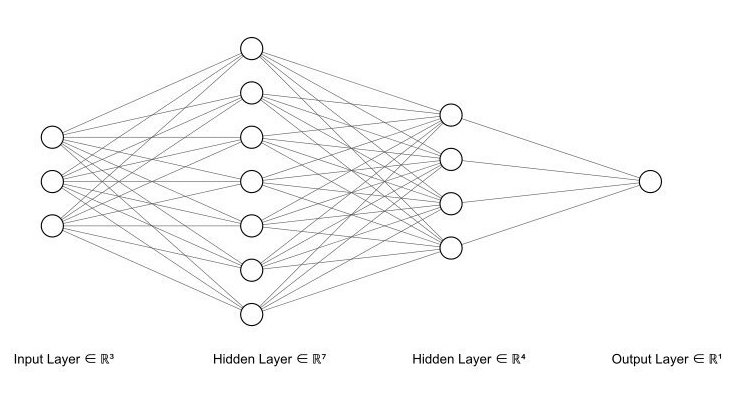
\includegraphics[width=\linewidth]{neural_net}
      \caption{A neural network with input $x\in \R^3$ and output $y\in\R$. The two hidden layers have dimensions $7$ and $4$ respectively. The graphic was generated with http://alexlenail.me/NN-SVG/index.html}\label{visual_nn}
	\end{minipage}
\end{center}
\end{figure}

\section{Training of neural networks}




\end{definition}
